
\chapter{Introduction}

In the field of pharmacology, drug discovery is the process through which new medications are brought to the market. To date, drug discovery is a highly expensive and difficult process with a low success rate, despite advances in technology and understanding of biological systems. Although the investment in drug research and development has increased substantially in recent years, the number of newly approved drugs by the US Food and Drug Administration (FDA) per year has not \cite{swinney2011were}. Since the sequencing of the human genome, the drug development process is mainly focused on proteins that are hypothesized to play a key role in diseases for which a drug is developed. Identifying chemical structures that modify the activity of these target proteins is a fundamental challenge in drug discovery. The most frequently used approach today is known as reverse pharmacology which involves large libraries of chemical compounds which need to be screened against the target proteins which are thought to be linked to the disease \cite{swinney2011were}. The identification of compounds which physically bind to the disease target is the key challenge here and thus  the knowledge about the interaction strength between chemical structures and proteins is an important topic in drug development. The safest and most accurate method to gain knowledge about the interaction strength of drug candidates and target proteins is through wetlab experiments. On the other hand, wetlab experiments are costly in terms of time and money, as there are thousands of potential drug candidates. The failure of a new ligand in toxicity tests is higher than $90\%$ which is the most significant reason for the high cost of the drug development process. 

In drug development, \textit{drug repositioning} is a technique in which known drugs and drug candidates are used to treat new diseases. Existing drugs may bind to the target protein of a disease other than the disease that the drug was originally developed for. Using an existing drug as a basis for the development of a new drug is far more likely to succeed, because the existing drug has already passed toxicity tests and its safety is known. Numerous openly accessible databases exist, listing the interaction of known compounds, which can be either already approved drugs or experimental drug candidates, against known target proteins (ChEMBL \cite{gaulton2012chembl}, DrugBank \cite{wishart2008drugbank}, KEGG\cite{kanehisa2011kegg}, SuperTarget \cite{gunther2008supertarget}, BindingDB \cite{liu2007bindingdb}). The high cost of in vitro methods for the testing of drug-target binding behaviour and the availability of experimental results in public databases give strong incentives to develop in silico methods for the prediction of new drug-target interactions. The development of a new model for this task is the topic of this thesis.

\section{Terms and Definitions}

Throughout this thesis the terms \textit{drugs} and \textit{targets} are used frequently. A simple introduction to these terms is given in this section.

\begin{itemize}
\item \textbf{Drugs:} In this thesis, the terms \textit{compounds} and \textit{drugs} are often used interchangeably. In drug discovery, a lead compound is a chemical structure that showed pharmacological activity that is likely to be therapeutically useful. The lead compound is used as a starting point which might be modified to increase the binding strength to the diseases target or to increase the selectivity with which it binds to the target. A high binding selectivity is important to reduce the potential side effects that the compound causes in the organism. The terms \textit{compounds} and \textit{drugs} are used interchangeably because the used datasets for the in silico prediction of drug-target interaction often contain both approved drugs and chemical structures that might be potential lead compounds. 
\item \textbf{Targets:} The terms \textit{target} and \textit{proteins} are often used interchangeably in this thesis. The identification of the biological origin of a disease is the first step in the discovery of a medicine. In a simplified formulation, certain proteins are hypothesized to be targets of intervention for the disease for which a drug is developed which changes the behavior or function of the respective proteins by physically binding to them. Here, the terms describe the proteins in the body whose activity can be modified by a drug through physical binding which causes a certain effect. The effect can be therapeutic if the drug binds to the targets of a disease or an unwanted side effect if the drug binds to other proteins.
\end{itemize}



\chapter{Review of Literature}
\label{chp:review}
Machine Learning and Data Mining techniques for drug development is a hot topic. In most existing methods the problem is formulated as a binary classification problem, where the drug-target pairs are treated as instances and the chemical structures of drugs and the amino acid subsequences of the targets are used as features, describing the instances. The goal in the binary formulation is to classify a given drug-target pair into binding and non binding. This approach stands in contrast with the developed method in this thesis, which predicts continuous drug-target binding affinities, where the binding affinity describes the strength of the binding between the drug and the target. The related methods which classify drug-target pairs will still be introduced here because the majority of existing work formulates the problem as such. Additionally, the only existing method in the literature, $KronRLS$, which predicts continuous binding affinities is introduced here. This method will be used as a comparison model to evaluate the developed model in this thesis. The following sections describe the state of the art machine learning based methods for drug-target interaction prediction, including the comparison model $KronRLS$. As described below, machine learning based methods for drug-target interaction prediction typically utilize similarity matrices of the drugs and targets to predict missing interactions. The method that is developed in this thesis follows this approach and the details of the types of similarity metrics for the drugs and targets are described in section \ref{sec:datasets}. To understand the related work, it is sufficient to know that a similarity value for each drug-drug pair and each target-target pair is given.

Two existing methods for drug-target interaction prediction that are not based on machine learning techniques are docking simulation and ligand-based approaches. In docking simulation the interaction strength of ligands and proteins is estimated based on the structure of the target protein. This process is extremely time-consuming and the structural information of a protein is not always available \cite{liu2016neighborhood}. In ligand based approaches, the interaction strength of a candidate ligand to a target protein is obtained by comparing the candiate ligand to ligands for which the interaction strength to the target is known. This approach is not applicable, when information of candidate-similar ligands is not available for the target protein. Both approches will not be examined further here. 

The following sections are titled by the first author of the respective method, followed by the title of the paper and the year that the method was published.

\section{Yoshihiro Yamanishi, "Prediction of drug-target interaction networks from the integration of chemical and genomic spaces.", 2008}

One of the first proposed models for the task \cite{yamanishi2008prediction}, is a supervised bipartite graph learning method. The motivation of the model is to reveal the correlations between drug similarity, target similarity and the drug-target interaction network. The authors define the \textit{chemical space} for drugs, the \textit{genomic space} for targets and the \textit{pharmacological space} for drug-target pairs and propose a method to embed compounds and proteins from the \textit{chemical} and \textit{genomic} spaces respectively into the unified \textit{pharmacological space}. New drug-target interactions are then predicted by connecting drugs and targets which are closer than a threshold in the \textit{pharmacological} space. 

In the authors model, the drug-target interaction network is represented by a bipartite graph $G=(V_1+V_2, E)$ , where $V_1$ is a set of drugs, $V_2$ is a set of target proteins and $E$ is a set of interactions between the drugs and targets. A graph-based similarity matrix 
$ K = \begin{pmatrix}

K_{cc} & K_{cg} \\
K_{cg}^T & K_{gg}
\end{pmatrix}
$
is constructed, where the elements of $K_{cc}$, $K_{gg}$, $K_{cg}$ are computed by using Gaussian functions:
$(K_{cc})_{ij}=exp(-d^2_{c_i,c_j}/h^2)$ for $i,j=1,\dots,n_c$, $(K_{gg})_{ij}=exp(-d^2_{g_ig_j}/h^2)$ for $i,j=1,\dots,n_g$ and $(K_{cg})_{ij} = exp(-d^2_{c_ig_j}/h^2)$ for $i=1,\dots,n_c, j=1,\dots,n_g$. Here $d$ stands for the shortest distance between two objects,  $n_c$ and $n_g$ stand for the number of known drugs and targets respectively and $h$ is a width parameter. 
To compute the vectors that span the \textit{pharmacological} space, the eigenvalue decomposition of $K$ is computed as:

$K=\Gamma \Lambda^{\frac{1}{2}} \Lambda^{\frac{1}{2}} \Gamma ^T = UU^T$ and all drugs and targets are represented by using the row vectors of the matrix $U=(u_{c_1},\dots,u_{c_{n_c}},u_{g_1},\dots,u_{g_{n_g}})^T$ .

Now two models are learned to map new compounds and targets from the \textit{chemical} and \textit{genomic} spaces respectively into the \textit{pharmacological} space. A kernel regression model that learns the feature vectors of new compounds and targets is proposed for this task:
\begin{center}
$u=\sum\limits_{i=1}^{n}s(x,x_i)w_i+\epsilon$
\end{center}

for the mapping of the compounds, $s(x,x_i)$ represents the compound similarity and for the mapping of the targets $s(x,x_i)$ represents the target similarity (and $n$ represents the number of drugs/targets in the training set). $\epsilon$ is a noise vector and $w_i$ is a weight vector that is learned by minimizing the loss function:
\begin{center}
$L=||UU^T - SWW^TS^T||^2_F$
\end{center}
where $S$ represents the respective similarity matrix, $W$ represents the matrix of weight vectors and $||.||_F$ represents the Frobenius norm.
Two such models, meaning two sets of weight vectors are learned to map new compounds and new targets onto the \textit{pharmacological} space.
Finally, based on the feature vectors $u$ in the \textit{pharmacological} space, feature-based similarity scores for three types of drug-target pairs are computed as the inner product as follows. 
\begin{itemize}
\item $corr(c_{new}, g_j) = u_{cnew}u_{gj}$
\item $corr(c_i, g_{new}) = u_{ci}u_{gnew}$
\item $corr(c_{new},g_{new}) = u_{cnew}u_{gnew}$
\end{itemize}
The three types of drug-target pairs, correspond to new drugs $c_{new}$ and known targets $g_j$, known drugs $c_i$ and new targets $g_{new}$ and new drugs and new targets $c_{new}$, $g_{new}$.
High-scoring compound-protein pairs of any of the three above types are predicted to interact with each other. Figure \ref{fig:yamanishi_1} illustrates the Supervised Bipartite Graph Inference Model.

\begin{figure}
\begin{center}
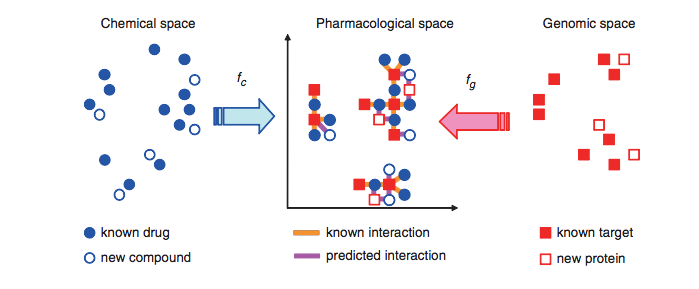
\includegraphics[scale=0.65]{yamanishi_related.png}
\end{center}
\caption[Illustration of Supervised Bipartite Graph Inference Method]{\large{Illustration of the Supervised Bipartite Graph Inference Model, \cite{yamanishi2008prediction}. All drugs and targets are mapped into the unified \textit{pharmacological} space. Similarity scores in the \textit{pharmacological} space for the drug-target pairs are then calculated as the inner product of the feature vectors.}}
\label{fig:yamanishi_1}
\end{figure}

\section{Twan van Laarhoven, "Gaussian interaction profile kernels for predicting drug-target interaction.", 2011}

The authors of this method first build an interaction profile for each drug and for each target. The interaction profile of each compound is a binary vector describing the presence or absence of interaction with every target in the network. The interaction profile for each target is defined analogously. Figure \ref{fig:laarhoven_1} illustrates the interaction profiles, constructed from the drug-target interaction network. The interaction profiles of the drugs and targets are used as feature vectors and a Gaussian kernel is constructed for the drugs and targets respectively. Let $y_{d_i}$ be the interaction profile of drug $d_i$, then the Gaussian kernel for the drugs is defined as
\begin{center}
$K_{GIP}(d_i,d_j) = exp(-\gamma_d || y_{di}-y_{dj} ||^2)$
\end{center}
and the Gaussian kernel for the targets can be defined analogously. Here, $GIP$ stands for Gaussian Interaction Profile and the parameter $\gamma_d$ controls the kernels bandwidth. The similarity information of the drugs and targets is integrated by defining two new kernels $K_{\text{chemical}}$ and $K_{\text{genomic}}$ for the drugs and targets respectively which are defined as:
\begin{equation}
\begin{split}
K_{\text{chemical}} = (S_D+S_D^T)/2 \\
K_{\text{genomic}} = (S_T+S_T^T)/2
\end{split}
\end{equation}
where $S_D$ and $S_T$ stand for the given similarity matrices of the drugs and targets. Finally, combined kernels of the two kernels $K_{GIP}$ and $K_{\text{chemical}}$/$K_{\text{genomic}}$ are defined as a weighted average:
\begin{center}
$K_d=\alpha_dK_{\text{chemical}}+(1-\alpha_d)K_{GIP}$\\
$K_t =\alpha_tK_{\text{genomic}}+(1-\alpha_t)K_{GIP}$
\end{center}
A Regularized Least Squares (RLS) classifier is chosen to generalize from the training data. The predicted values $\hat{y}$ of the RLS classifier for a given kernel $K$ and training vector $y$ are defined as:
\begin{center}
$\hat{y} = K(K+\sigma I)^{-1}y$
\end{center}
With the matrix $Y\in n_d \times n_t$ being the binary matrix of training values of $n_d$ drugs and $n_t$ targets and the kernels for the drugs and targets as defined above, the authors of the model propose two ways to predict the interaction of all drug-target pairs in the matrix. The first type of prediction $RLS$-$avg$ is defined as:
\begin{center}
$\hat{Y}=\frac{1}{2}(K_d(K_d+\sigma I)^{-1}Y)+\frac{1}{2}(K_t(K_t+\sigma I)^{-1}Y^T)^T$
\end{center}
For the second type of prediction, the authors propose to compute yet a fourth kernel, defined by the Kronecker product $K = K_d \otimes K_t$, which gives a similarity for all drug-target pairs. The model named \textit{RLS-Kron} predicts $\hat{Y}$ as:
\begin{center}
$vec(\hat{Y}^T) = K(K+\sigma I)^{-1}vec(Y^T)$
\end{center}


\begin{figure}
\begin{center}
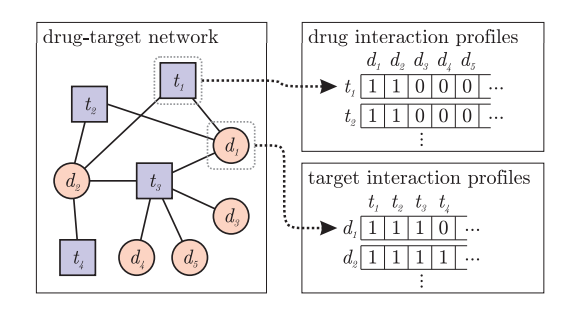
\includegraphics[scale=0.65]{laarhoven_related.png}
\end{center}
\caption[Illustration of Gaussian Interaction Profile Kernel Method]{\large{Illustration of the interaction profiles, constructed from the drug-target interaction network.}}
\label{fig:laarhoven_1}
\end{figure}

\section{Fan Yang, "Drug-target interaction prediction by integrating chemical, genomic, functional and pharmacological data.", 2014}

This method is introduced here because it is the only method in the literature that also utilizes Conditional Random Fields to predict drug-target interaction. The authors propose the following model to classify drug-target pairs into binding or non-binding: Let $\{d_i\}$ be the set of known drugs and $\{t_j\}$ be the set of known targets. $X$ is used to denote the known drug-target interactions and the similarity information among the drugs and targets. For each drug $d_i$ an undirected graph $G=(V_t, E_t)$ is defined, where $V_t=\{t_j\}$ is the set of targets and each edge in $E_t$ represents the similarity between a pair of targets. Let $Y=(y_1, y_2, \dots, y_{n_t})$, where $n_t$ is the total number of known targets, denote the prediction, where each $y_j$ is a binary random variable representing the prediction on target $t_j$, that is, $y_j=1$ if the predicted interaction between $d_i$ and target $t_j$ is true, and $y_j=0$ otherwise. These graphs will in the following be referred to as the target-based CRFs. Similarly, an undirected graph $G=(V_d, E_d)$, where $V_d$ is the set of known drugs and $E_d$ represents the similarity between a pair of drugs is constructed for each target. These graphs will in the following be referred to as the drug-based CRFs. 

In order to predict the interaction of all drugs, using the target-based CRFs, a joint probability distribution which is conditioned on the observation $X$ is defined for each target-based CRF, meaning a separate CRF is constructed for each drug. In the underlying graph, each node represents a target $t_i$ and its associated binary random variable $y_i$, and each edge connecting two nodes represents the dependency between these two nodes. The energy of a joint configuration $Y$, given $X$ for any of the target-based CRFs is defined as follows:

\begin{equation}
E(Y|X) = \sum\limits_{i} a_i f(y_i|X) + \sum\limits_{i,j} b_{ij}g(y_i, y_j | X)
\end{equation}

where $f(y_i|X)$ is a local node feature function defined based on the state of $y_i$, $g(y_i, y_j | X)$ is a relational edge feature function defined based on states of both $y_i$ and $y_j$ and $a_i\geq 0$ and $b_{ij} \geq 0$ are weight parameters that are learned from training data. The functions $f$ and $g$ are defined as follows:
\begin{equation}
f(y_i|X) = -(y_i - H_{xi}(y_i))^2
\end{equation}
\begin{equation}
g(y_i,y_j | X) = -H_{x_i,x_j}(y_i-y_j)^2
\end{equation}
where $H_{xi}(y_i)$ represents the observed feature of target $t_i$. In the authors implementation, $H_{xi}(y_i)$ is the average number of observed drug interactions for target $t_i$. $H_{x_i,x_j}(y_i-y_j)$ denotes the difference between binary variables $y_i$ and $y_j$. Intuitively, this formulation adds a penalization when predictions for two similar nodes are different and when the prediction of a given node deviates from its average state.
The authors of the method let all target-based CRFs share the same parameters $a_i$ and $b_{ij}$ and similarly for all drug-based CRFs. The joint probability density function of $Y$ given $X$ is then defined as:

\begin{equation}
P(Y|X) = \frac{1}{Z(X)}\text{exp}(-E(Y|X))
\end{equation}

where $Z(X)=\sum\limits_{Y}exp(-E(Y|X))$ is the partition function of the CRF. As described in \cite{yang2014drug}, the parameters can be learned by optimizing the log-likelihood of the training data by stochastic gradient ascent. To predict unknown drug-target interactions for a query drug and target $t_k$, the conditional probability $p(y_k|y_{-k},X)$ can be computed for each target $t_k$, where $t_{-k}$ denotes all other targets except $t_k$. The conditional expectation of $y_k$ is calculated as the prediction score of the interaction between target $t_k$ and the query drug. Similarly, a prediction score can be computed for a query target and each drug. A weighted average of the drug-based and the target-based CRFs is taken as the final prediction for each drug-target pair in the authors implementation.



\section{Yong Liu, "Neighborhood Regularized Logistic Matrix Factorization for Drug-Target Interaction Prediction", 2016}
The study \cite{liu2016neighborhood} proposes a method named Neighborhood Regularized Logistic Matrix Factorization (NRLMF) for the task of drug-target interaction prediction which predicts the probability that a drug would interact with a target. In this method, the properties of a drug and a target are represented by two latent vectors in a shared low dimensional latent space. The interaction probability of a drug-target pair is modeled by a logistic function of the drug-specific and the target-specific latent vectors. In the learning step, regularization constraints between the latent representations of similar drugs and targets are applied, such that similar latent vectors are learned for similar drugs and targets. Formally, the problem is described as follows: The set of known drugs is denoted by $D=\{d_i\}$, with $i=1,\dots,m$ and the set of known targets is denoted by $T=\{t_j\}$, $j=1,\dots,n$, where $m$ and $n$ are the number of drugs and targets, respectively. In addition, the drug similarities are represented by $S^d \in \mathbb{R}^{m \times m}$ and the target similarities by $S^t \in \mathbb{R}^{n \times n}$. A binary matrix $Y \in \mathbb{R}^{m \times n}$, where each element $y_{ij}\in \{0,1\}$ is given as training data. If drug $d_i$ has been experimentally verified to interact with target $t_j$, $y_{ij}$ is set to $1$ and otherwise $y_{ij}$ is set to $0$. Both, the drugs and the targets are mapped into a shared latent space, with a low dimensionality $r$. The properties of a drug $d_i$ and a target $t_j$ are described by two latent vectors $u_i \in \mathbb{R}^{1 \times r}$ and $v_j \in \mathbb{R}^{1\times r}$, respectively. The interaction probability $p_{ij}$ of a drug-target pair $(d_i, t_j)$ is then modeled by the logistic function:
\begin{equation}
\label{eq:blabla}
p_{ij}=\frac{\text{exp}(u_i v_j^T)}{1+\text{exp}(u_iv_j^T)}
\end{equation}
In the following, let $U\in \mathbb{R}^{m \times r}$ and $V \in \mathbb{R}^{n \times r}$ denote the latent vectors of all drugs and targets respectively, such that $u_i$ is the $i^{th}$ row in $U$ and $v_j$ is the $j^{th}$ row in $V$. 
Under the assumption that all training examples are independant, the probability of the observations in the training matrix $Y$ is:
\begin{equation}
\begin{split}
& p(Y|U,V) = \\
& \big(\prod\limits_{1\leq i \leq m, 1\leq j \leq n, y_{ij}=1} [p_{ij}^{y_{ij}} (1-p_{ij})^{(1-y_{ij})}]^c \big)\times \big(\prod\limits_{1\leq i \leq m, 1\leq j \leq n, y_{ij}=0} p_{ij}^{y_{ij}}(1-p_{ij})^{(1-y_{ij})} \big)
\end{split}
\end{equation}
where $c$ is a constant used to control the importance levels of observed interactions. This importance weighting strategy is used to assign higher importance to positive interactions, because the positive interactions are biologically validated and thus more trustworthy. The negative interactions in contrast could contain potential drug-target interactions and are thus unreliable.

As derived in \cite{liu2016neighborhood}, the model parameters $U$ and $V$ can be learned by maximizing the posterior distribution, which is equivalent to minimizing the following objective function:
\begin{equation}
\label{eq:bla}
\min\limits_{U,V}= \sum\limits_{i=1}^{m} \sum\limits_{j=1}^{n} (1+cy_{ij}-y_{ij})\text{log}[1+\text{exp}(u_iv_j^T)] - cy_{ij}u_iv_j^T + \frac{\lambda_d}{2}||U||^2_F+\frac{\lambda_t}{2}||V||^2_F
\end{equation}
where $\lambda_d=\frac{1}{\sigma^2_d}$ and $\lambda_t=\frac{1}{\sigma^2_t}$ are parameters controlling the variances of Gaussian priors on the latent vectors of the drugs and targets and $||.||_F$ denotes the Frobenius norm.

Next, the drug and target similarities are integrated as follows: For drug $d_i$, let $N(d_i)$ denote the $K_1$ most similar drugs to $d_i$ and analogously let $N(t_j)$ denote the $K_2$ most similar targets to $t_j$. The drug neighborhood information is represented using an adjacency matrix $A$, where the $(i,y)$ element $a_{iy}$ is defined as:
\begin{equation}
a_{iy} = \begin{cases}
S^d_{iy} & \text{if }  d_y \in N(d_i) \\
0 & \text{otherwise} 
\end{cases}
\end{equation}
and similarly the target neighborhood information is denoted by $B$, where its $(j,x)$ element $b_{jx}$ is defined as:
\begin{equation}
b_{jx} = \begin{cases}
S^t_{jx} & \text{if } t_x \in N(t_j) \\
0 & \text{otherwise} 
\end{cases}
\end{equation}

Now, intuitively the drug and target similarities are integrated by adding constraints such that the distance of the latent vectors between each drug/target $d_i$/$t_j$ and its nearest neighbors $N(d_i)$/$N(t_j)$ is minimized. This can be achieved by adding constraining terms to the objective function. For the drugs, the constraining term has the following form:
\begin{equation}
\frac{\alpha}{2}\sum\limits_{i=1}^{m}\sum\limits_{y=1}^{m}a_{iy}||u_i - u_y||_F^2
\end{equation}
A similar term is added for the latent vectors of the targets. These constraining terms are added to the objective function \ref{eq:bla} to integrate the similarity metrics. The full derivation and the resulting objective function which minimizes the posterior distribution including the constraining terms is shown in \cite{liu2016neighborhood}. Once the latent vectors $U$ and $V$ have been learned, the probability associated with any unknown drug-target pair $(d_i, t_j)$ can be predicted by equation \ref{eq:blabla}. In \cite{liu2016neighborhood} the drugs and targets are further distinguished into drugs/targets with known interactions and drugs/targets without any known interaction. These details are left out here.

\section{Tapio Pahikkala, "Toward more realistic drug-target interaction predictions.", 2014}

$KronRLS$ is a model for continuous drug-target interaction prediction that was presented in \cite{pahikkala2014toward}. The model that is developed in this thesis will later be compared to the performance of $KronRLS$. $KronRLS$ is a kernel methods which formulates the problem as follows:
for a set $D$ of drugs and a set $T$ of targets, we have a set $X = x_1,\dots,x_m$ of drug-target pairs ($X$ is a subset of $D\times T$) with an associated vector $y = y_1,\dots,y_m$ of continuous binding affinities as training data. To find a prediction function $f(x)$ for all possible drug-target pairs $x \in D\times T$, we learn $f$ from the training data by minimizing the objective:
\begin{equation}
J(f) = \sum\limits_{i=1}^{m}(y_i-f(x_i))^2 + \lambda ||f||_k^2
\end{equation}
In the objective function, $||f||_k^2$ is the norm of $f$, which is associated to a kernel function $k$ (which is described below), and $\lambda>0$ is a user defined regularization parameter. A minimizer of the above objective can be expressed as 
\begin{equation}
\label{eq:blablabla}
f(x)=\sum\limits_{i=1}^
{m} a_i k(x,x_i)
\end{equation}
The kernel function $k$ is a symmetric similarity measure between each of the $m$ drug-target pairs, which can be represented by a $m \times m$ matrix $K$. When we have two individual similarity matrices $K_d$ and $K_t$ for the drugs and targets respectively, a similarity matrix for each drug-target pair can be computed as \mbox{$K_d \otimes K_t$}, where $\otimes$ stands for the Kronecker product. We can see that intuitively, the parameters $a$ represent how much can be interpolated from each known drug-target pair.

Now we first assume that the training set $X$ contains every possible pair of drugs and targets (which is not the case in the real application of the method). With this assumption, we can compute $K$ as \mbox{$K = K_d \otimes K_t$} and we can learn the parameters $a_i$ which define the minimizer $f$ by solving the system of linear equations:
\begin{equation}
(K+\lambda I)a = y
\end{equation} where $I$ is the $D\times T$ identity matrix. 
For the real world scenario, where only a subset of $D\times T$ is given as training data, the vector $y$ has missing values in the above formulation. To find the parameters $a$,  \cite{pahikkala2014toward} suggests to formulate the problem as above and use approaches such as conjugate gradient, combined with Kronecker algebraic optimization to solve the system of linear equations.

Finally, predictions for all drug-target pairs of all drugs and targets that appear in the training data can be made through equation \ref{eq:blablabla}.



